\documentclass{article} % For LaTeX2e
\usepackage{nips15submit_e,times}
\usepackage{hyperref}
\usepackage{url}
\usepackage{amssymb,amsmath}
\usepackage[pdftex]{graphicx}
\usepackage{algorithm}
\usepackage{algpseudocode}
%\documentstyle[nips14submit_09,times,art10]{article} % For LaTeX 2.09


\title{Variational Bayesian Inference for Neural Feature Tagging of Unstructured Stimuli}


\author{
John M.~Pearson\\
Duke Institute for Brain Sciences \\
Duke University\\
Durham, NC 27708 \\
\texttt{john.pearson@duke.edu} \\
\And
Jeffrey M.~Beck \\
Department of Neurobiology \\
Duke University Medical Center \\
Durham, NC 27708 \\
\texttt{jeff.beck@duke.edu} \\
}

\newcommand{\fix}{\marginpar{FIX}}
\newcommand{\new}{\marginpar{NEW}}

% \nipsfinalcopy % Uncomment for camera-ready version

\begin{document}

\maketitle

\begin{abstract}
Experiments that study neural encoding of stimuli at the level of individual neurons typically choose a small set of features present in the world --- contrast and luminance for vision, pitch and intensity for sound --- and assemble a stimulus set that systematically (and preferably exhaustively) varies along these dimensions. Neuronal responses in the form of firing rates are then examined for modulation with respect to these features via some form of regression. This approach requires that experimenters know (or guess) in advance the relevant features coded by a given population of neurons. Unfortunately, for domains as complex as social interaction or natural movement, the relevant feature space is poorly understood, and an arbitrary \emph{a priori} choice of feature sets may give rise to confirmation bias. Here, we present a Bayesian model for exploratory data analysis that is capable of automatically identifying the features present in unstructured stimuli based solely on neuronal responses. Our approach is unique within the class of latent state space models of neural activity in that it assumes that firing rates of neurons are sensitive to multiple discrete time-varying features, each of which has Markov (or semi-Markov) dynamics. We derive a fast variational Bayesian inference algorithm and show that it correctly recovers hidden features in synthetic data, as well as ground-truth stimulus features in a prototypical neural dataset. To demonstrate the utility of the algorithm, we also apply it to an exploratory analysis of prefrontal cortex recordings performed while monkeys watched naturalistic videos of primate social activity.
\end{abstract}

\section{Introduction}
The question of how the brain encodes information from the natural world forms one of the primary areas of study within neuroscience. For many sensory systems, particularly vision and audition, the discovery that single neurons modulate their firing of action potentials in response to particular stimulus features has proven foundational for theories of sensory function. Indeed, neuronal responses to contrast, edges, and motion direction appear to form fundamental primitives on which higher-level visual abstractions are built. Nevertheless, many of these higher-level abstractions, increasingly of interested to modern neuroscience, do not exist in a stimulus space with obvious axes. As a result, experimentalists must choose \emph{a priori} features of interest in constructing their stimulus sets, with the result that cells may appear broadly and weakly tuned due to misalignment of stimulus and neural axes.

For example, in vision, methods like reverse correlation have proven successful in elucidating response properties of some cell types, but such techniques rely on a well-behaved stimulus space and a highly constrained encoding model in order to achieve sufficient statistical power to perform inference \cite{steveninck1988realtime,ringach2004reverse,ringach2002receptive}. However, natural stimuli are known to violate both criteria, and generate receptive fields and patterns of neural activity that differ markedly from those observed in controlled experiments with limited stimulus complexity \cite{ringach2002receptive,sharpee2004analyzing,Vinje2000-dx}. Information-based approaches have gone some way in addressing this challenge \cite{sharpee2004analyzing}, but this approach assumes a metric structure on stimuli in order to optimize encoded information, and was recently shown to be strongly related to standard Poisson regression models\cite{Williamson2013-rg}.

More recently, Gallant and collaborators have tackled this problem in the context of fMRI, demonstrating that information present in the blood oxygen level-dependent (BOLD) signal is sufficient to classify and map the representation of natural movie stimuli across the brain \cite{Kay2008-gd,Vu2011-da,Huth2012-cj,Stansbury2013-nm}. These studies have used a number of modeling frameworks, from latent dirichlet allocation for categorizing scene contents \cite{Stansbury2013-nm} to regularized linear regression \cite{Huth2012-cj} to sparse nonparametric models \cite{Vu2011-da} to characterize brain encoding of stimuli, but in each case, models were built on pre-labeled training data. Clearly, a method that could infer stimulus structure directly from neural data themselves could extend such work to include less easily characterized stimulus sets like those depicting social interactions.

Another recent line of work, this one focused on latent Poisson processes, has addressed the task of modeling the low dimensional dynamics of neural populations\cite{Pillow2008-em,Vogelstein2009-ax,Park2014-el,Buesing2014-ta}. Using generalized linear models and latent linear dynamical systems as building blocks, these models have proven able to infer (functional) connectivity \cite{Pillow2008-em}, estimate spike times from a calcium images\cite{Vogelstein2009-ax}, and identify subgroups of neurons that share response dynamics\cite{Buesing2014-ta}. Inference in thsese models is generally performed via expectation maximization, though \cite{Ulrich2014-zc} and \cite{Putzky2014-up} also used a variational Bayesian approach. Our work is distinct from those models, however, in that both were concerned with modeling and discriminating \emph{internal} states based on neural responses, while this work focuses on detecting features in \emph{external} stimuli. 

Our model sits at the intersection of these regression and latent variable approaches. We utilize a Poisson observation model that shares many of the same features as the commonly used generalized linear models for Poisson regression. We also assumes that the latent features which modulate neural activity are time-varying and Markov. Uniquely, however, we (1) assume that the activity of each neuron is modulated by a combination of multiple independent latent features governed by semi-Markov dynamics and (2) enforce a sparse hierarchical prior on modulation strength that effectively limits the number of latent features to which any given neuron is selective. The semi-Markov assumption allows for latents to evolve over multiple timescales with non-trivial duration distributions much like the hand-labeled features in social interaction data sets. Additionally, the sparse prior allows for a parsimonious explanation of firing rates of single units in terms of a small set of features. Finally, we use variational Bayesian methods and take advantage of conditional conjugacy to generate coordinate ascent update rules (almost all of which are explicit) for all model parameters. Combined with forward-backward inference for latent states, our algorithm is exceptionally fast, automatically implements Occam's razor, and facilitates proper model comparisons using the variational lower bound.   

\section{Model}
\label{model_sec}
\begin{figure}[ht]
    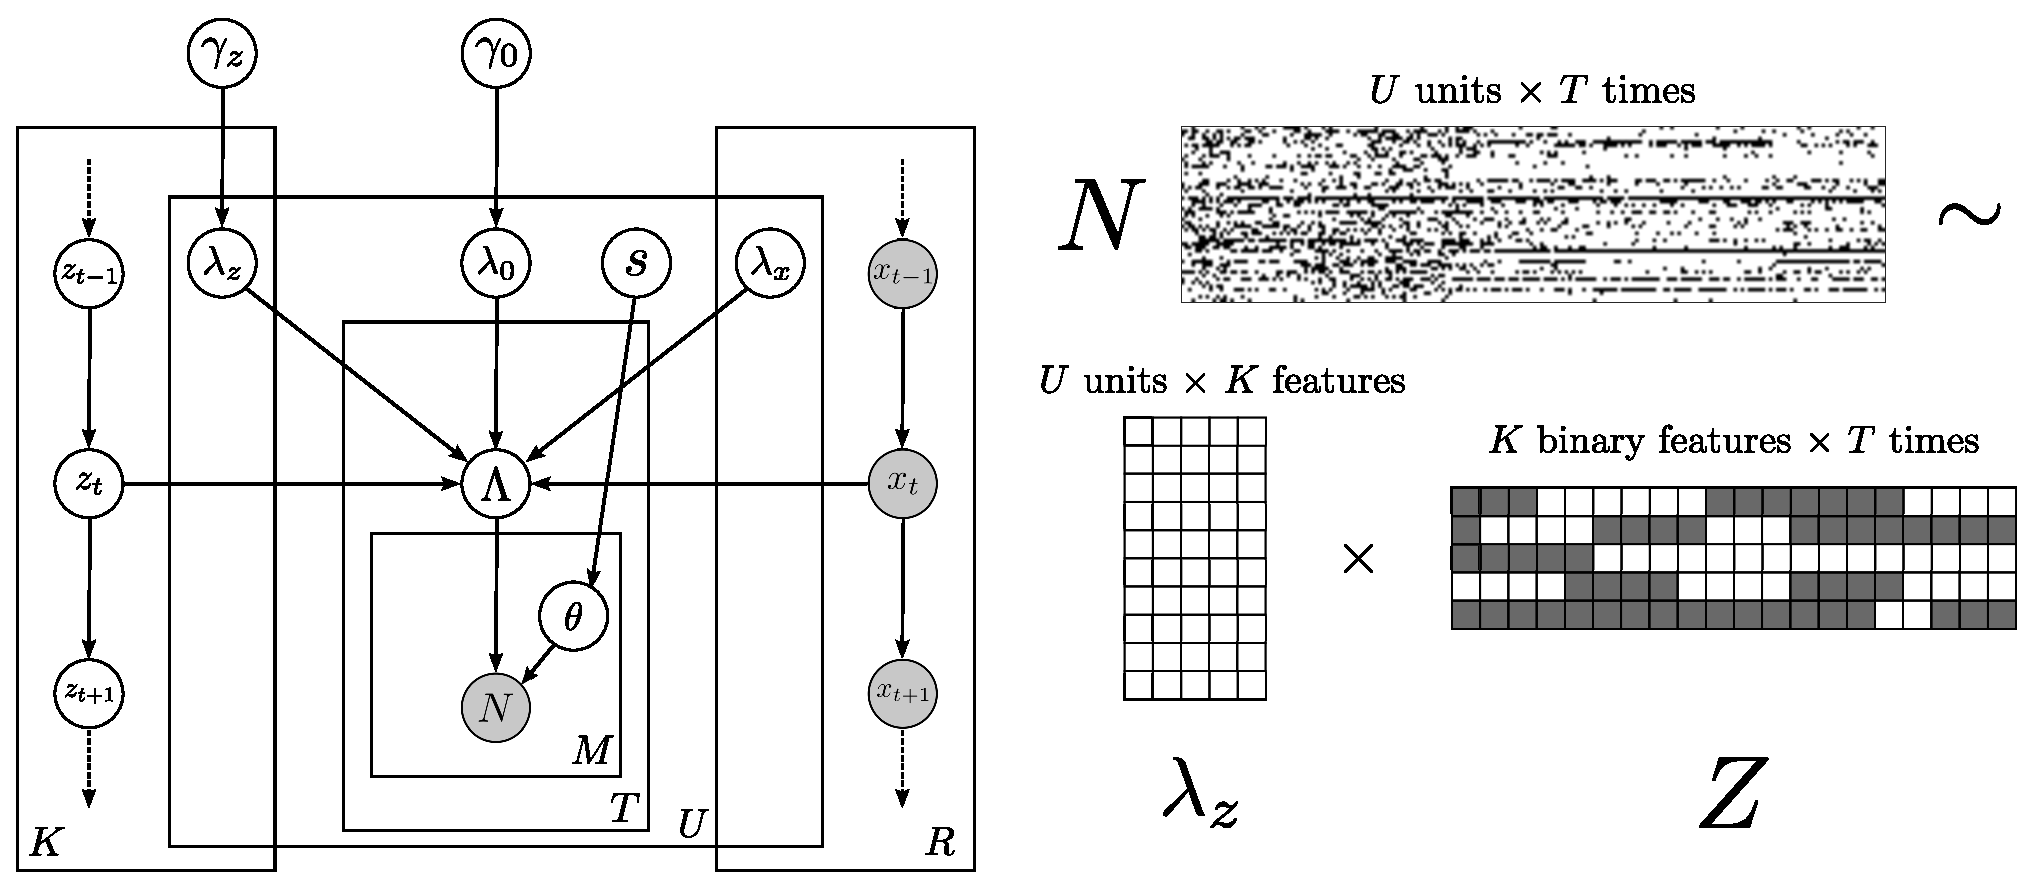
\includegraphics[width=1\linewidth]{figures/model}
    \caption{\textbf{Generative model for spike counts.} Spike counts $N$ are observed for each of $U$ units over stimulus time $T$ for multiple presentations $M$. Counts are assumed Poisson-distributed, with firing rates $\Lambda$ that depend on each unit's responses ($\lambda$) to both latent discrete states $z_t$ and observed covariates $x_t$ that change in time, as well as a baseline firing rate $\lambda_0$. $\gamma$ nodes represent hyperparameters for the firing rate effects. $\theta$ is a multiplicative overdispersion term specific to each observation, distributed according to hyperparameters $s$.}
\end{figure}
\subsection{Observation model}
Consider a population of $U$ spiking neurons exposed to a series of stimuli indexed by a (unique) time index $t\in \lbrace 1\ldots T\rbrace$. Moreover, each neuron is exposed to each stimulus $M_{tu}$ times, where we do not assume either that each neuron observes each stimulus time or that consecutive times are observed by the same sets of neurons. That is $M_{tu}$ may have many 0s. For each observation $m$ (a unique unit, time pair), we then observe a spike count, $N_m$. We model these spike counts as arising from a Poisson process with time-dependent rate $\Lambda_{tu}$ and observation-specific multiplicative overdispersion $\theta_m$:
\begin{align}
    \label{obs_model}
    N_{m} &\sim \text{Pois}(\Lambda_{t(m), u(m)} \theta_m) &
    \theta_m &\sim \text{Ga}(s_{u(m)}, s_{u(m)})
\end{align}
Note that both the unit and time are functions of the observation index, $m$, and that the distribution of the overdispersion for each observation is specific to the unit observed. 

\subsection{Firing rate model}
At each stimulus time $t$, we assume the existence of $K$ binary latent states $z_{tk}$ and $R$ observed covariates $x_{tr}$. We further assume that each unit's firing rate response at each time can be modeled as arising from the product of three effects: (1) a baseline firing rate specific to each unit, (2) a product of responses to each latent state, and (3) a product of responses to each observed covariate:
\begin{equation}
    \label{fr_model}
    \Lambda_{tu} = \lambda_{0u} \prod_{k = 1}^K \lambda_{zuk}^{z_{tk}}  
    \prod_{r = 1}^R \lambda_{xur}^{x_{tr}}   
\end{equation} 
Note that this is conceptually similar to the generalized linear model for firing rates (in which we model $\log \Lambda$) with the identification $\beta = \log \lambda$. However, by modeling the firing rate directly as a product and placing Gamma priors on the individual effects, we will be able to take advantage of closed-form variational updates resulting from conjugacy that avoid explicit optimization in the case of the $z$s (see below). 

In addition, to enforce parsimony in the inferred features, we put sparse hierarchical priors with hyperparameters $\gamma = (c, d)$ on the $\lambda_z$ terms:
\begin{align}
    \label{hierarchy}
    \lambda_{zuk} &\sim \text{Ga}(c_{zk}, c_{zk} d_{zk}) & c_{zk} &\sim \text{Ga}(a_{ck}, b_{ck})
    & d_{zk} &\sim \text{Ga}(a_{dk}, b_{dk})
\end{align}
That is, $\mathbb{E}[\lambda_u] = d^{-1}$ and $\text{var}[\lambda_u] = (cd^2)^{-1}$, so for $c$ large and $d\sim \mathcal{O}(1)$, the prior for firing rate response to each latent feature will be strongly concentrated around 0. And once again, this choice of priors will lead to closed-form updates in our variational approximation. Finally, for the baseline terms, $\lambda_{0u}$, we use a non-sparse version of the same model, while for the specified covariate responses, $\lambda_{xu}$, we model the unit effects non-hierarchially using independent Gamma priors for each unit.

\subsection{Latent state model}
We model the latent states $z_{tk}$ as an independent Hidden Markov Model (HMM) for each feature $k$. That is, each $k$ indexes an independent Markov chain with initial state probability $\pi_k$ and transition matrix $A_k$. For the semi-Markov case, we assume that the dwell times in each state are distributed independently for each chain according to an integer-valued, truncated lognormal distribution with maximum duration $D$:
\begin{align}
    \label{semi-markov}
    p_k(d|z = j) &= \text{Log-Normal}(d|m_{jk}, s^2_{jk}) / W_{jk}  &
    W_{jk} &= \sum_{d = 1}^D \text{Log-Normal}(d|m_{jk}, s^2_{jk}) 
\end{align}
where we have allowed the dwell time distribution to depend on both the feature $k$ and the state of the Markov chain $j$. In addition, we put indpendent Normal-Gamma priors on the mean $(m_{kj})$ and precision $(\tau_{kj} \equiv s_{kj}^{-2})$ parameters of the distribution: $(m, \tau) \sim \text{NG}(\mu, \lambda, \alpha, \beta)$.

\section{Inference}

\begin{algorithm}[ht]
\caption{Iterative update for variational inference}\label{algo}
\begin{algorithmic}[1]
\Procedure{Iterate}{}
    \State Update baselines $\lambda_0$\Comment{conjugate Gamma}
    \State Update baseline hyperparameters $\gamma_0$\Comment{conjugate Gamma}
    \For{$k = 1\ldots K$}\Comment{always in the same order}
        \State Update firing rate effects $\lambda_{zk}$\Comment{conjugate Gamma}
        \State Update firing rate hyperparameters $\gamma_{zk}$\Comment{conjugate Gamma}
        \State Update Markov chain parameters $A_k, \pi_k$
        \State $z_k$ posteriors $\gets$\Call{forward-backward}{}
        \If{semi-Markov}
            \State Update duration distribution $p_k(d|j)$\Comment{BFGS optimization}
            \State Update duration hyperparameters
        \EndIf
    \EndFor
    \State Update covariate firing effects $\lambda_x$\Comment{BFGS optimization}
    \State Update overdispersion $\theta$\Comment{conjugate Gamma}
\EndProcedure
\end{algorithmic}
\end{algorithm}

We perform variational inference for the posteriors over the model variables $\Theta = (\lambda_0, \lambda_z, \lambda_x, z, A, \pi, \theta, c_0, d_0, c_z, d_z, s)$. In addition, for the semi-Markov case, we include variables $(m, \tau)$, the parameters for the state dwell time distribution. That is, we wish to approximate the joint posterior density, 
\begin{equation}
    p(\Theta|N) \propto p(N, z|\lambda, A, \pi, \theta, \gamma) 
    p(\lambda|\gamma) p(\gamma)
    p(A)p(\pi)p(\theta|s)p(s)
\end{equation}
by a variational posterior $q(\Theta)$ that is closest to $p$ as measured by the Kullback-Leibler divergence \cite{Wainwright2008-ii}. Equivalently, we wish to maximize the variational objective
\begin{equation}
    \mathcal{L} \equiv \mathbb{E}_q \left[\log \frac{p(\Theta|N)}{q(\Theta)} \right] = \mathbb{E}_q \left[\log p(\Theta|N) \right] + \mathcal{H}[q(\Theta)]
\end{equation}
with $\mathcal{H}$ the entropy of the variational posterior. For the form of our variational posterior, we take a quasi-mean field approximation in which the posterior factorizes over units and latent and observed factors, but not time. That is, it forms a factorial HMM \cite{ghahramani1997factorial}:
\begin{multline}
    q(\Theta) = q(c_0)q(d_0)\prod_m q(\theta_m) \prod_u q(s_u) q(\lambda_{0u}) \prod_r q(\lambda_{xur}) \times \\ 
    \prod_k q(c_k) q(d_k) 
    q(\lambda_{zuk}) q(c_{zk}) q(d_{zk}) q(z_k) q(\pi_k) q(A_k)
\end{multline}
With this ansatz, the variational objective decomposes in a natural way, and choices are available for many of the $q$s that lead to closed-form updates.

\subsection{Variational posterior}
From \ref{obs_model} and \ref{fr_model} above, we can write the probability of the observed data $N$ as
\begin{multline}
    \label{log_evidence}
    \log p(N, z|x, \Theta) = \sum_{mkr} \left[ 
        N_m \left( \log \theta_m +
            \log \lambda_{0u(m)} +
            z_{t(m) k} \log \lambda_{zu(m) k} + 
            x_{t(m) r} \log \lambda_{xu(m) r}
            \right)
    \right] \\
    - \sum_m \theta_m \Lambda_{t(m) u(m)} + 
    \sum_{mk} \log (A_k)_{z_{t(m)+1, k}, z_{t(m), k}} + 
    \sum_k \log (\pi_k)_{z_{0k}} + \text{constant,}
\end{multline}
where again, $m$ indexes observations of (time, unit) pairs and the last two nontrivial terms represent the probability of the Markov sequence given by $z_{tk}$. Given that \ref{log_evidence} is of an exponential family form for $\theta$ and $\lambda$ conditioned on all other variables, free-form variational arguments \cite{Blei2006-oh} suggest variational posteriors:
\begin{align}
    \lambda_{0u} &\sim \text{Ga}(\alpha_{0u}, \beta_{0u}) &
    \lambda_{zuk} &\sim \text{Ga}(\alpha_{zuk}, \beta_{zuk}) &
    \lambda_{xur} &\sim \text{Ga}(\alpha_{xur}, \beta_{xur})
\end{align}
For the first of these two, updates in terms of expected sufficient statistics involving expectations of $\gamma = (c, d)$ are straightforward (see Supplement). However, this relies on the fact that $z_t \in \lbrace0, 1\rbrace$. The observed covariates $x_t$ follow no such restriction, which results in a transcendental equation for the $\beta_x$ updates which we solve using an explicit BFGS optimization on each iteration. Moreover, we place non-hierarchical Gamma priors on these effects: $\lambda_{xur} \sim \text{Ga}(a_{xur}, b_{xur})$.

As stated above, we place hierarchical priors on $\lambda_0$, $\lambda_z$, and $\theta$ of the form \ref{hierarchy}\footnote{This hierarchy is over units for $\lambda$ and over observations for $\theta$.}. This involves multiple terms in the expected log evidence of the form
\begin{equation}
    \mathbb{E}_q \left[\sum_u \log p(\lambda_u|c, d)\right] = \sum_u \mathbb{E}_q \left[ 
    (c - 1) \log \lambda_u - cd\lambda_u + c \log cd - \log \Gamma(c) 
    \right] 
\end{equation}
In order to calculate the expectation, we make use of the inequality %\cite{abramowitz1964handbook}
\begin{equation}
    \sqrt{2\pi} \le \frac{z!}{z^{z+\frac{1}{2}} e^{-z}} \le e
\end{equation}
to lower bound the negative gamma function and approximate the above as
\begin{equation}
    \log p(\lambda) \ge \sum_u \left[ 
    (c - 1) (\log \lambda_u + 1) - cd\lambda_u + c \log d + \frac{1}{2}\log c\right]
\end{equation}
Clearly, the conditional probabilities for $c$ and $d$ are gamma in form, so that if we use priors $c \sim \text{Ga}(a_c, b_c)$ and $d\sim \text{Ga}(a_d, b_d)$ the posteriors have the form
\begin{align}
    c &\sim \text{Ga}\left(a_c + \frac{U}{2}, 
    b_c + \sum_u\mathbb{E}_q 
        \left[d \lambda_u - \log \lambda_u - \log d - 1\right]\right) \\
    d &\sim \text{Ga}\left(
        a_d + U\mathbb{E}_q[c], b_d + \sum_u \mathbb{E}_q [c \lambda_u]
    \right)
\end{align}
This basic form, with appropriate indices added, gives the update rules for the hyperparameter posteriors for $\lambda_0$ and $\lambda_z$. For $\theta$, we simply set $c = s_u$ and $d = 1$.

\subsection{Latent state inference}
For Hidden Markov Models, given the observation model \ref{log_evidence}, inference for $z$, $A$, and $\pi$ for each latent feature can be performed efficiently via conjugate updates and the well-known forward-backward algorithm \cite{beal2003variational}. We do not randomize the order of chain updates on each iteration of Algorithm \ref{algo}. For the case of semi-Markov dynamics, we additionally need to perform inference on the parameters $(m, \tau)$ of the dwell time distributions for each state. In the case of continuous dwell times, our model \ref{semi-markov} would have $W = 1$ and be conjugate to the Normal-Gamma prior on $(m, \tau)$, but the restriction to discrete dwell times requires us to again lower bound the variational objective:
\begin{equation}
    \mathbb{E}_q\left[-\log W_{jk} \right] = 
    \mathbb{E}_q\left[- \log \left( \sum_{d=1}^D p(d|j)\right) \right]
    \ge -\log \sum_{d = 1}^D \mathbb{E}_q\left[p(d|j)\right]
\end{equation}
This correction for trunction must then be added to $\mathbb{E}_q[p(z|\Theta)]$. For inference in this case, we use an extension of the forward-backward algorithm to semi-Markov transitions \cite{Yu2006-bb}, at the expense of time complexity $\mathcal{O}(SDT)$ $(S = 2)$ per latent state, to calculate $q(z_k)$ (see Supplement). For the $4SK$ hyperparameters of the Normal-Gamma distribution, we perform an explicit BFGS optimization on the $4S$ parameters of each chain on each iteration.

\section{Experiments}
\subsection{Synthetic data}
We generated synthetic data from the model in Section \ref{model_sec} for $U=100$ neurons for $T=10,000$ time bins of $dt=0.0333s$ ($\approx 6$min). Assumed firing rates and effect sizes were realistic for cortical neurons, with mean baseline rates of 10 spikes/s and firing rate effects given by a $\text{Ga}(1, 1)$ distribution for $K_{\text{data}}=3$ latent features. In addition, we included $R=3$ known covariates generated according to Markov dynamics. For this experiment, we assumed that each unit was presented once with the stimulus time series, so that $M = 1$. That is, we tested a case in which inference was driven primarily by variabiliy in population responses across stimuli rather than pooling of data across repetitions of the same stimulus. Moreover, to test the model's ability to parsimoniously infer features, we set $K=5$. That is, we asked the model to recover more features than were present in the data.

As discussed above, we placed hierarchical priors on unit baseline firing rates and sparse hierarchical priors on firing rate effects of latent states. We used 5 random restarts and iterated over parameter updates until the fractional change in $\mathcal{L}$ dropped below $10^{-4}$.

\begin{figure}[ht]
    \center
    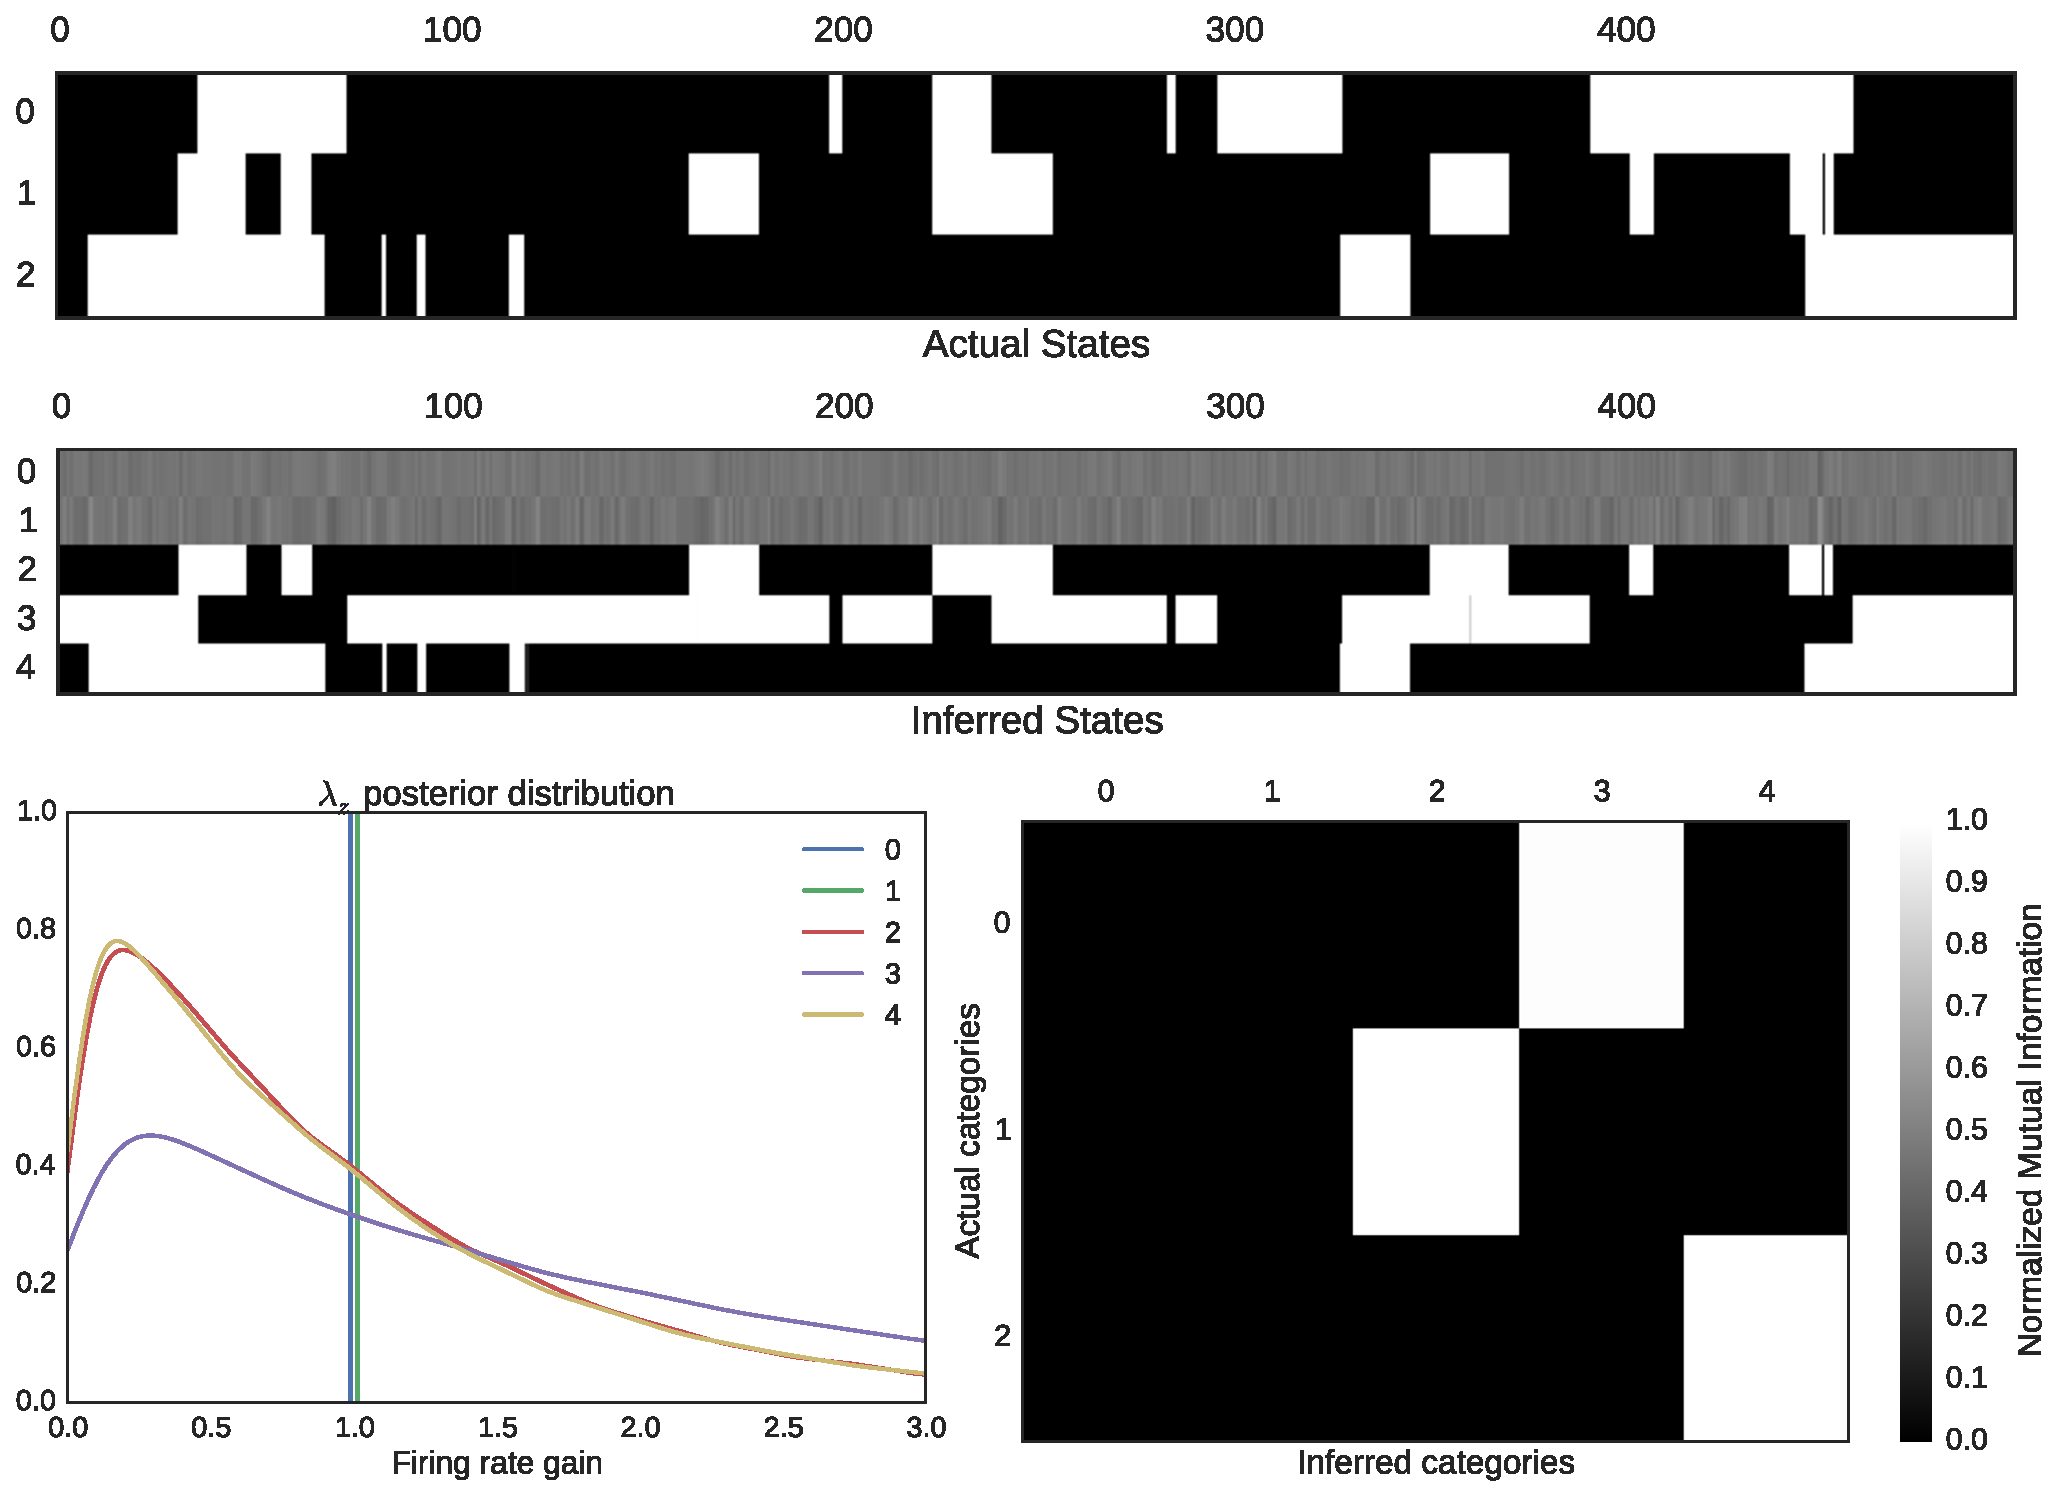
\includegraphics[width=0.6\linewidth]{figures/synthetic}
    \caption{\textbf{Top:} Actual and recovered binary features for a subset of stimulus times in the dataset. Note that inferred feature 3 is the inverse of actual feature 0, and that unused features are in gray, indicating a high posterior uncertainty in the model. \textbf{Bottom left:} Population posterior distributions for $\lambda_z$. Features 0 and 1 are effectively point masses around gain 1 (no effect), while features 2--4 approximate the $\text{Ga}(1, 1)$ data-generating model. \textbf{Bottom right:} Normalized mutual information between actual and inferred states.}
    \label{synthetic}
\end{figure}

As seen in Figure \ref{synthetic}, the model correctly recovers only the features present in the original data. We quantified this by calculating the normalized mutual information $\hat{I}\equiv I(X, Y)/\sqrt{H(X)H(Y)}$, between the actual states and the inferred states, with $H(Z)$ and $I$ estimated by averaging the variational posteriors (both absolute and conditioned on actual states) across time. Note that superfluous features in the model have high posterior uncertainty for $z_k$ and high posterior confidence for $\lambda_{zk}$ around 1 (no effect). In addition, the model correctly recovers coefficients for the observed covariates, and when limited to fewer features than in the generating model, recovers a subset of the features accurately rather than blending features together (see Supplement).

\subsection{Labeled neural data}
We applied our model to a well-studied neural data set comprising single neuron recordings from macaque area LIP during the performance of a perceptual discrimination task \cite{roitman2002response}\footnote{Data available at \texttt{https://www.shadlenlab.columbia.edu/resources/RoitmanDataCode.html}}. In the experiment, stimuli consisting of moving dots of different levels of coherence were shown to the animals, whose task it was to report the direction of motion. Moreover, on each trial, one direction was favored, in that the location of the target indicating this direction was placed in the response field of the recorded neuron. Thus, in addition to 5 coherence levels, each trial also varied based on whether the motion direction corresponed to the target in or out of the response field.

We fit a model with $K = 10$ features and $U = 27$ units to neural responses from the 1-second stimulus presentation period of the task. Spike counts corresponded to bins of $dt = 20$ms. In this case, each unit experienced a different number of presentations of each stimulus condition, resulting in a ragged observation matrix.

\begin{figure}[ht]
    \center
    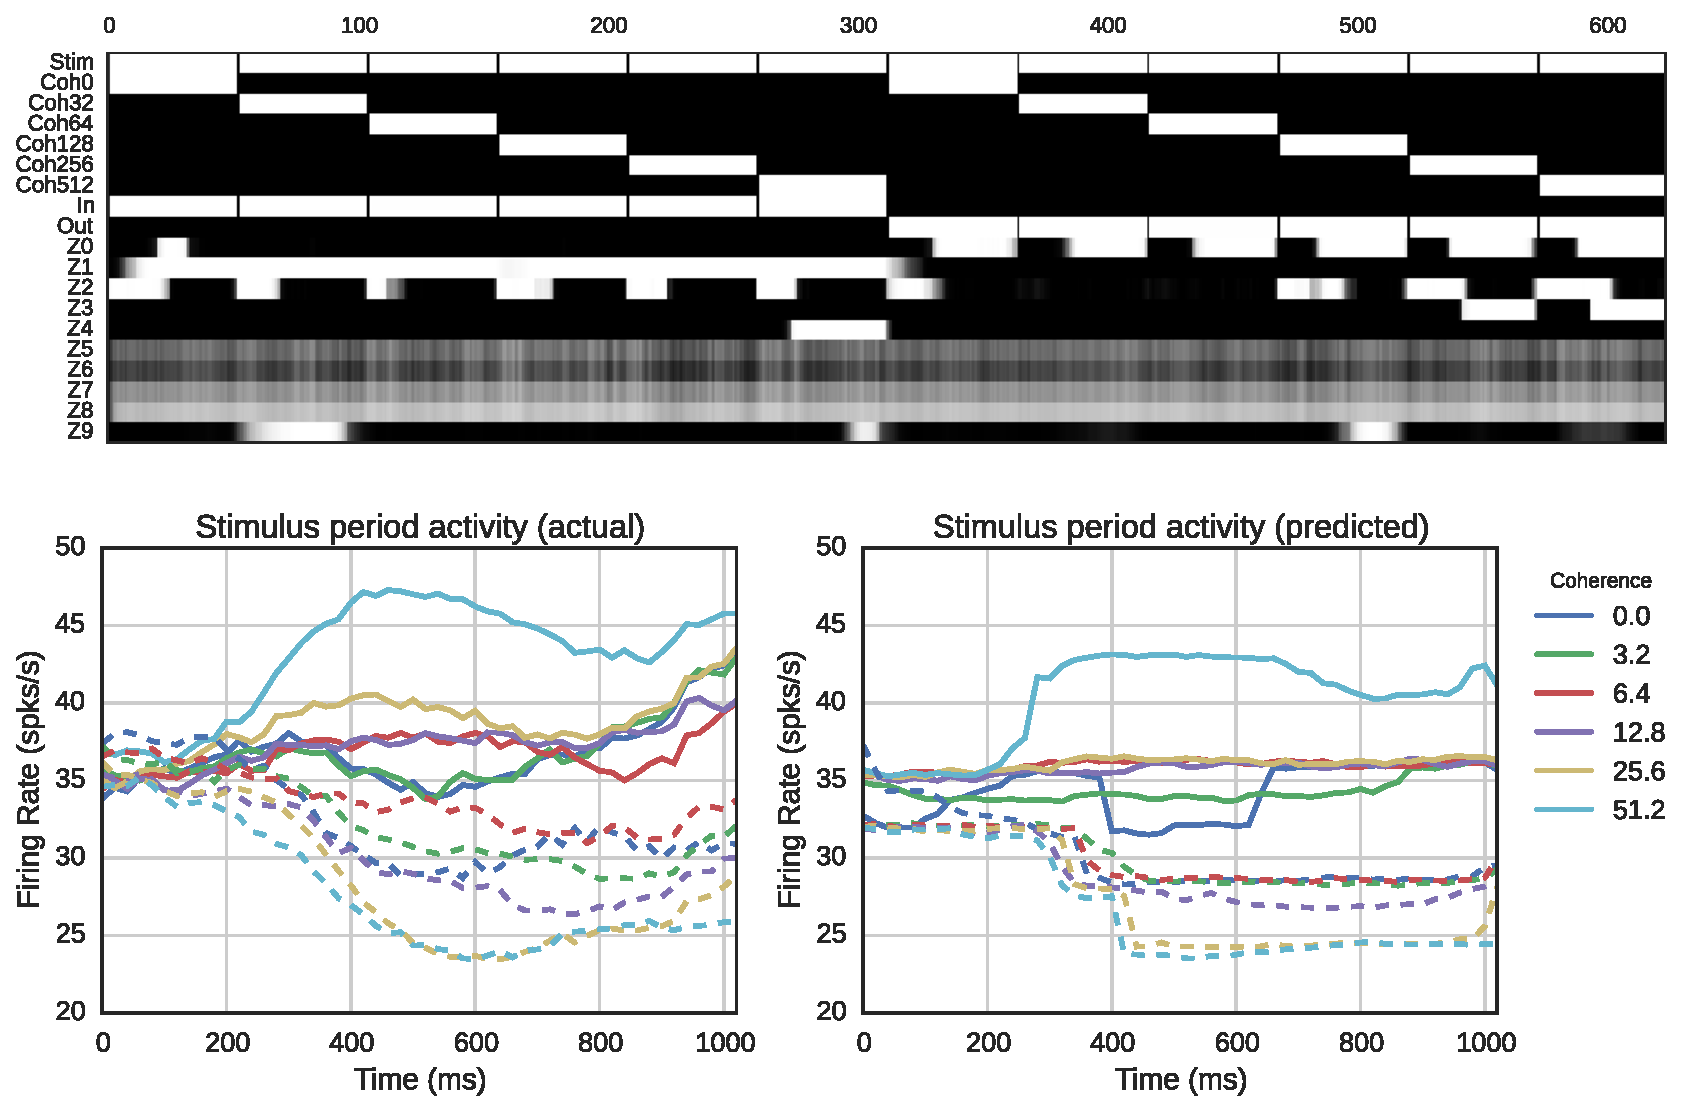
\includegraphics[width=0.7\linewidth]{figures/roitman}
    \caption{\textbf{Top:} Actual and recovered binary features during the stimulus presentation period. Note that model features 5 -- 8 are unused and that feature 0 closely tracks the Out feature of the data, albeit delayed. \textbf{Bottom} Actual and predicted firing rates for the stimulus period. Note that the model infers stimulus categories from the data, including appropriate timing of differences between categories.}
    \label{roitman}
\end{figure}
Figure \ref{roitman} shows the experimental labels from the concatenated stimulus periods, along with labels inferred by our model. Once again, the model has left some features unused, but correctly discerned differences in between stimuli in the unlabeled data. Even more importantly, though given ten distinct stimulus classes, the model has clearly inferred the factorial design of the experiment, with the two most prominent features, $z_0$ and $z_1$, corresponding to the two levels of the crossed factor with the largest effect size: whether or not the relevant target is inside or outside the receptive field of the neuron. In addition the model correctly captures the initial 200ms ``dead time'' during the stimulus period in which firing rates remain at pre-stimulus baseline. In addition, the model groups stimuli with similar firing rates together, as well as roughly capturing the time course of stimulus differentiation. As a result, mismatch between the ground truth labels and model-inferred features reflects fundamental ambiguities in the neural data, with the model's latent states taking into account features of spiking response not necessarily known in advance by experimenters.

\subsection{Movie data}
Finally, we applied our model to a data set comprising single neuron recordings made in macaque monkeys as they freely viewed movies of primate social interactions in the wild %\cite{adams_inprep}
 . These video clips, collected from a rhesus macaque research field site, represent the range of behaviorally relevant stimuli for this common primate experimental model species, particularly the four ``F''s of animal behavior: fighting, fleeing, foraging, and reproduction. Thus this dataset represents a rare opportunity for exploratory feature selection based on neural responses.

On each trial of the experiment, monkeys viewed a random 5-second clip from a movie database ($T \approx 5$h, $dt = 30$ frames/s). On the following trial, monkeys were given a two-alternative choices with options chosen from the set \{repeat clip, continue clip, blank screen, new clip\}. Since each neuron saw only a subset of clips within the database, and these clips began at with random offsets, observations were sparse, with total number of observations $N_{obs} = 7.42 \times 10^6$ and $\overline{M} = N_{obs}/T \approx 14$. These data form a particularly intriguing application of our model, since the neurons recorded were located in the orbitofrontal and dorsolateral prefrontal cortices, areas not normally associated with low-level visual processing. In fact, there is reason to believe that the relevant features encoded in these areas for such naturalistic stimuli are behavioral and social \cite{watson2012social}.

Because the behaviors of interest in these stimuli potentially span a large range of time scales, we used semi-Markov dynamics with a maximum duration of $D = 500$ on the latent states\footnote{We also allowed for self-transitions, potentially capturing behavior on even longer timescales.}. We fit a model with $K=10$ features and the same hierarchical priors on baselines and latent firing rate effects as in previous experiments. In addition, because many neurons in the data set exhibited a transitory increase in firing with movie onset on each trial (independent of movie content), we include this movie onset response as an external covariate $x(t)$ for each neuron. We calculated this separately for each recorded unit by averaging spike counts (relative to stimulus onset) across trials, smoothing, and taking the log so that $x(t)$ was coded as a multiplicative rather than an additive effect on firing. This can be loosely viewed as a means of ``pre-whitening'' our data, in which we remove a large nuisance regressor by specifying it as a covariate in the model.

\textbf{One paragraph of results discussion for Experiment 3}

\textbf{Figure 3 about here}

\section{Discussion}
Here, we have proposed and implemented a method for learning features in stimuli via the responses of populations of spiking neurons. This work addresses a growing trend in systems neuroscience --- the increasing use of rich and unstructured stimulus sets --- without requiring either expert labeling or a metric on the stimulus space. As such, we expect it to be of particular use in disciplines like social neuroscience, olfaction, and other areas in which the real world is complex and strong hypotheses about the forms of the neural code are lacking. By learning features of interest to neural populations directly from data, we stand to generate unexpected, more accurate hypotheses about the brain's relationship to the sensory world.

We have shown that our model is capable of parsimoniously and correctly inferring features in the low signal-to-noise regime of cortical activity, even in the case of indpendently recorded neurons. Moreover, by employing a Variational Bayesian approach to inference, we gain three key advantages: First, we gain the advantages of Bayesianism in general: estimates of confidence in inferences, parsimony and regularization via priors, and the ability to do principled model comparison. Second variational methods, particularly those using stochastic gradient approaches, scale well to large datasets. Finally, variational methods are fast, in that they typically converge within only a few tens of iterations and in many case (such as ours) require mostly simple algebraic coordinate updates. Combined with the modularity of this and similar approaches, such models provide a promising opportunity to ``build out'' additional features that will meet the challenges of the next generation of experimental data.



\subsubsection*{Acknowledgments}
%This work was supported by an NIH Big Data to Knowledge Career Development Award to JP (K01ES025442).


\newpage
\subsubsection*{References}
\begingroup
\renewcommand{\section}[2]{}
\bibliography{pearson_beck}{}
\bibliographystyle{ieeetr}
\endgroup

\end{document}
